\documentclass[conference]{IEEEtran}
\IEEEoverridecommandlockouts

\usepackage[utf8]{inputenc}
\usepackage[T1]{fontenc}
\usepackage[english]{babel}
\usepackage{cite}
\usepackage{amsmath,amssymb}
\usepackage{graphicx}
\usepackage[table]{xcolor}
\usepackage[section]{placeins}
\usepackage{url}
\definecolor{tokenpackhighlight}{RGB}{226,241,255}

\title{TokenPack: Modeling LLM Context Window Selection as a 0/1 Knapsack Problem}

\author{
\IEEEauthorblockN{Metehan Kizilcik}
\IEEEauthorblockA{
Department of Software Engineering\\
HFTTF\\
Email: 232803055@ogr.cbu.edu.tr}
}

\begin{document}
\maketitle

\begin{abstract}
Large language models cannot always process full long documents because their context windows are limited. This project models context selection as a 0/1 Knapsack Problem. Each semantic text chunk is treated as an item, its token count is treated as weight, and its semantic similarity to the query is treated as value. The implemented prototype, TokenPack, compares naive top-k retrieval, budget-aware top-k retrieval, MMR, value-based greedy selection, density-based greedy selection, simulated annealing, random feasible selection, and dynamic-programming-based knapsack selection. To fit the Algorithm Analysis and Design course objective, the experiments are repeated 100 times for each problem size and report average value, runtime, accuracy gap, confidence interval, and timeout rate. Results show that exact dynamic programming gives the optimum for manageable instances, but becomes impractical as the $nC$ state space grows. Greedy density is much faster and usually close to optimum, while value-only greedy can have a large accuracy gap. The retrieval experiment also shows why plain top-k is unsafe for LLM systems: it can exceed the context budget even when the retrieved chunks are relevant.
\end{abstract}

\begin{IEEEkeywords}
Knapsack, 0/1 Knapsack, Greedy Algorithm, Dynamic Programming, LLM, RAG, Context Window, Algorithm Analysis
\end{IEEEkeywords}

\section{Introduction}
NP-Hard problems such as the Traveling Salesman Problem, Warehouse Location Problem, and Knapsack Problem are commonly used in algorithm analysis courses to compare exact and heuristic algorithms. This project applies the 0/1 Knapsack Problem to a modern setting: context window selection for large language models (LLMs).

When a long document is divided into candidate chunks, only a subset can be placed into the limited token budget of an LLM. This selection task naturally follows a knapsack structure. TokenPack models the context window as a capacity, text chunks as items, token counts as weights, and query relevance scores as values.

The central research question is: can a classical NP-Hard optimization model improve LLM context selection compared with retrieval heuristics that only rank chunks independently? This question is important because LLM context windows are expensive and finite resources. A chunk with high semantic relevance but very large token cost may not be the best choice if several shorter chunks collectively provide more useful evidence. Therefore, the problem is not only a retrieval problem; it is a constrained optimization problem.

The contribution of this project is threefold. First, it presents a direct mapping between LLM context selection and the 0/1 Knapsack Problem. Second, it implements exact and heuristic algorithms in a reusable Python package and command-line tool. Third, it evaluates these algorithms using repeated synthetic experiments, a small retrieval feasibility benchmark, and a pilot LLM answer-quality/cost analysis.

\section{Literature Review}
The Knapsack Problem is one of the fundamental NP-Hard problems in combinatorial optimization \cite{karp1972reducibility,martello1990knapsack}. Many extensions and solution strategies have been studied, including multidimensional, multiobjective, and multiple-choice variants \cite{cacchiani2022recent,lust2010multiobjective,szkaliczki2025mckp}. Metaheuristic optimization methods such as NSGA-II are also frequently used for combinatorial optimization when exact methods are too expensive \cite{verma2021nsga}.

Retrieval-Augmented Generation (RAG) provides external knowledge to LLMs by retrieving relevant document chunks \cite{lewis2020rag}. However, simple top-k retrieval does not directly optimize token budget usage. Long-context methods such as MemGPT, Parallel Context Windows, LongRoPE, PoSE, and positional interpolation show that context length is a major practical limitation in LLM systems \cite{packer2023memgpt,ratner2023pcw,ding2024longrope,zhu2023pose,chen2023positional}. Recent evaluations also compare long-context models and RAG, and show that effective context length and computational cost still matter even when nominal context windows grow \cite{xu2023retrieval,li2024longcontextrag,paulsen2025effective,ahmed2025optimization}.

Chunking and embedding quality are also central to retrieval. Late Chunking, S2 Chunking, Landmark Embedding, and document chunking studies demonstrate that segmentation and representation choices affect downstream retrieval quality \cite{gunther2024latechunking,verma2025s2chunking,luo2024landmark,luo2024bge,documentchunking2026}. Context pruning and query-aware sparsity methods such as AttentionRAG, Quest, SnapKV, WindowKV, and BudgetMem further support the idea that not every token should be placed into the model context \cite{attentionrag2025,tang2024quest,li2024snapkv,zuo2025windowkv,budgetmem2025}.

Knapsack-style formulations have also appeared in summarization and recent LLM optimization work. Tree knapsack summarization and budget-aware summarization explicitly connect content selection with budget constraints \cite{hirao2013treeknapsack,pilault2022factorizing}. Recent LLM-oriented work uses knapsack-like ideas for NP-Hard problem evaluation, exploration budget allocation, and speculative decoding \cite{duchnowski2025knapsack,li2025knapsackrl,cha2026knapspec}. TokenPack follows this direction but focuses specifically on retrieval-time context packing.

\section{Problem Formulation}
Given a query $q$, a document is split into $n$ chunks. Each chunk $i$ has a value $v_i$ and a weight $w_i$. In TokenPack, $v_i$ is computed from cosine similarity between the query embedding and chunk embedding, while $w_i$ is the chunk token count. The effective LLM context budget is denoted by $C$.

The optimization problem is:

\begin{equation}
\max \sum_{i=1}^{n} v_i x_i
\end{equation}

\begin{equation}
\sum_{i=1}^{n} w_i x_i \leq C,\quad x_i \in \{0,1\}
\end{equation}

Here, $x_i=1$ means that chunk $i$ is selected. The objective maximizes total semantic utility while preserving the hard token budget. This formulation is more suitable than top-k retrieval when chunk lengths are unequal, because top-k ignores item weight.

\section{Method}
The TokenPack pipeline has four main stages:

\begin{enumerate}
  \item The long document is split into chunks using paragraph-group or semantic-threshold chunking.
  \item Each chunk and query is embedded into a vector space.
  \item Chunk value is computed using cosine similarity, and chunk weight is computed using token count.
  \item Selection is performed with top-k, budget-top-k, MMR, greedy heuristics, or 0/1 knapsack dynamic programming.
\end{enumerate}

\subsection{Semantic Chunking}
Chunking is the stage that converts an unstructured long document into knapsack items. This is important because the optimization algorithm can only choose among the chunks that the preprocessing stage creates. If chunk boundaries are poor, even an optimal knapsack solver may select incomplete or semantically broken evidence.

TokenPack supports two chunking modes. The first mode is \textbf{paragraph-group chunking}. The document is first split into structural blocks such as paragraphs or PDF text blocks. Consecutive blocks are then grouped until the chunk reaches a target token range. In this project, the intended range is approximately 400--900 tokens. This keeps chunks large enough to preserve local context, but small enough for the optimizer to combine several pieces under a limited context budget. Each chunk keeps metadata such as source path, page number when available, block order, and character offsets. This metadata is important because selected chunks are later restored to their original document order before being sent to the LLM.

The second mode is \textbf{semantic-threshold chunking}. Instead of grouping only by length, this mode compares neighboring text blocks in embedding space. For two adjacent blocks $b_i$ and $b_{i+1}$, TokenPack computes:

\begin{equation}
s_i = \cos(E(b_i), E(b_{i+1}))
\end{equation}

where $E(\cdot)$ is the embedding function. If $s_i$ falls below a threshold, the algorithm treats this point as a topic shift and starts a new chunk. A maximum token limit is still enforced, so semantic chunking cannot create chunks that violate the later token-budget assumptions. This makes the chunker both semantic and budget-aware.

The purpose of semantic chunking is not to solve the optimization problem by itself. Instead, it improves the quality of the item set given to knapsack. Paragraph grouping provides stable and explainable boundaries, while semantic-threshold chunking can split documents at topic changes. In both cases, the output item must contain three values needed by the optimizer: text content, token weight, and source-order metadata.

\subsection{Compared Algorithms}
\textbf{Dynamic Programming (DP).} DP computes the optimal subset under the token capacity. The implementation uses a one-dimensional value table for the objective and a reconstruction table for selected weight. Its time complexity is $O(nC)$.

\textbf{Greedy by Value.} This heuristic sorts chunks by value and inserts each chunk if it fits. It is fast, but it may choose large chunks that block better combinations.

\textbf{Greedy by Value Density.} This heuristic sorts chunks by $v_i/w_i$. It is usually stronger than value-only greedy because it accounts for token efficiency, but it is still not guaranteed to find the optimal 0/1 solution.

\textbf{Greedy by Lightest Weight.} This baseline chooses short chunks first. It tests whether token minimization alone is enough. In practice, it ignores semantic value and therefore may select weak evidence.

\textbf{Random Feasible.} This baseline shuffles chunks and inserts feasible items. It gives a lower-bound style comparison for non-optimized selection.

\textbf{Simulated Annealing (SA).} SA starts from a density-greedy feasible solution and then explores neighboring subsets by adding or removing one item at a time. Worse moves can be accepted with a probability controlled by a decreasing temperature. This gives a metaheuristic baseline that is closer to the course project examples than simple greedy selection.

\textbf{Document-prefix and Full-document Baselines.} These two baselines represent the system without TokenPack-style optimization. Document-prefix inserts chunks in the original PDF order until the budget is full. Full-document tries to insert the entire source document. These baselines are useful because they show what happens when semantic value and token cost are not optimized jointly.

\textbf{Top-k, Budget-top-k, and MMR.} Top-k selects a fixed number of chunks only by similarity. Budget-top-k adds a feasibility check. MMR additionally penalizes redundancy between selected chunks.

These algorithms were not only described theoretically; they were executed on the same generated instances so that their differences can be measured statistically. Table \ref{tab:algorithm-comparison} reports a paired comparison for $N=1000$ over 100 runs. The word ``paired'' means that every algorithm receives the same item values, weights, and capacity for each repetition. Therefore, the measured gap is caused by the algorithmic strategy rather than by different random inputs. In the tables, shaded rows mark the TokenPack-relevant exact knapsack baseline and its practical density-based heuristic.

\begin{table}[!t]
\caption{Paired Statistical Comparison of Algorithms for $N=1000$ over 100 Runs}
\label{tab:algorithm-comparison}
\centering
\scriptsize
\resizebox{\columnwidth}{!}{%
\begin{tabular}{lrrrrr}
\hline
Algorithm & Mean Value & Mean Time (ms) & Gap (\%) & 95\% CI Gap & Speedup \\
\hline
\rowcolor{tokenpackhighlight}\textbf{DP exact} & 111281.2 & 56.644 & 0.00 & 0.00 & -- \\
\rowcolor{tokenpackhighlight}\textbf{Greedy density} & 111252.4 & 0.209 & 0.03 & 0.01 & 271.3x \\
Simulated annealing & 111252.4 & 3.784 & 0.03 & 0.01 & 15.0x \\
Greedy lightest & 95924.7 & 0.150 & 13.84 & 0.38 & 376.4x \\
Greedy value & 40785.1 & 0.147 & 63.30 & 0.65 & 386.4x \\
Random feasible & 20897.2 & 0.173 & 81.20 & 0.43 & 326.8x \\
\hline
\end{tabular}%
}
\end{table}


The comparison shows a clear trade-off. DP is the exact baseline and has zero gap, but it is much slower. Greedy density is approximately 271 times faster than DP in this setting while keeping the mean gap at only 0.03\%. Simulated annealing reaches a similar gap in this experiment, but it is slower than density-greedy because it performs additional neighborhood exploration. Greedy value is also fast, but its mean gap is 63.30\%, which shows that choosing high-value items without considering weight is unreliable. The lightest-first baseline is faster than DP but loses 13.84\% value on average, proving that minimizing tokens alone is also not enough.
\FloatBarrier

\subsection{Why Knapsack is Appropriate}
The mapping from context selection to knapsack is direct. The context window is the capacity, chunks are items, token counts are weights, and query relevance scores are values. This model is more faithful than top-k because it optimizes total information value under an explicit constraint. It also supports fair algorithm analysis: exact DP can be compared with greedy heuristics using runtime, timeout rate, and accuracy gap.

\section{Complexity Analysis}
For $n$ candidate chunks and effective token budget $C$, the DP algorithm has $O(nC)$ time complexity. This is pseudo-polynomial: it is efficient for moderate token budgets but can become expensive when either the number of chunks or the capacity is large. Greedy algorithms require sorting, so their time complexity is $O(n \log n)$ and memory usage is low.

This theoretical expectation leads to a practical hybrid design. Embedding similarity first prunes the candidate pool, then a knapsack optimizer is applied only to the strongest candidates. This keeps DP feasible while preserving the main advantage of exact budget-aware optimization.

\section{Experimental Design}
Three experiments are used.

\textbf{Repeated synthetic knapsack benchmark.} Random instances are generated for $N \in \{100,500,1000,5000,10000\}$. Each setting is repeated 100 times with different random seeds. DP is treated as the exact baseline when $nC \leq 5{,}000{,}000$ states. For larger instances, DP is marked as timeout to represent the practical point where the exact method becomes too expensive. The reported metrics are mean objective value, mean runtime, standard deviation of runtime, mean accuracy gap from DP optimum, maximum gap, and timeout rate.

\textbf{Retrieval feasibility benchmark.} A small human-reviewed gold-evidence benchmark checks whether retrieval strategies obey the token budget. This benchmark compares no-optimization baselines, top-k, budget-top-k, MMR, and knapsack on selected document chunks. Its purpose is not to prove final QA quality, but to verify the main engineering constraint: a context selection algorithm must not exceed the budget.

\textbf{LLM answer-quality and cost pilot.} The reviewed gold questions are also sent to local Ollama models and a cloud LLM after context selection. The small model is Qwen3 0.6B, the medium model is Qwen3 4B, and the large cloud model is OpenAI GPT-4o. Cloud credentials are read from a local \texttt{OPENAI\_API\_KEY} environment variable, and no key is stored in the repository. The answer scores are automatic lexical pilot scores, not final human judgments. Cost is estimated by scaling average selected input tokens to a 1M baseline-token scenario using public API pricing assumptions \cite{openaipricing2026}.

\section{Experimental Results}
Figure \ref{fig:runtime-scaling} visualizes the runtime behavior of the compared algorithms. The y-axis is logarithmic because DP and greedy methods operate at very different time scales. DP grows much faster as $N$ increases, while greedy methods remain almost flat in comparison. This matches the theoretical difference between $O(nC)$ dynamic programming and $O(n\log n)$ greedy sorting.

\begin{figure}[!t]
\centering
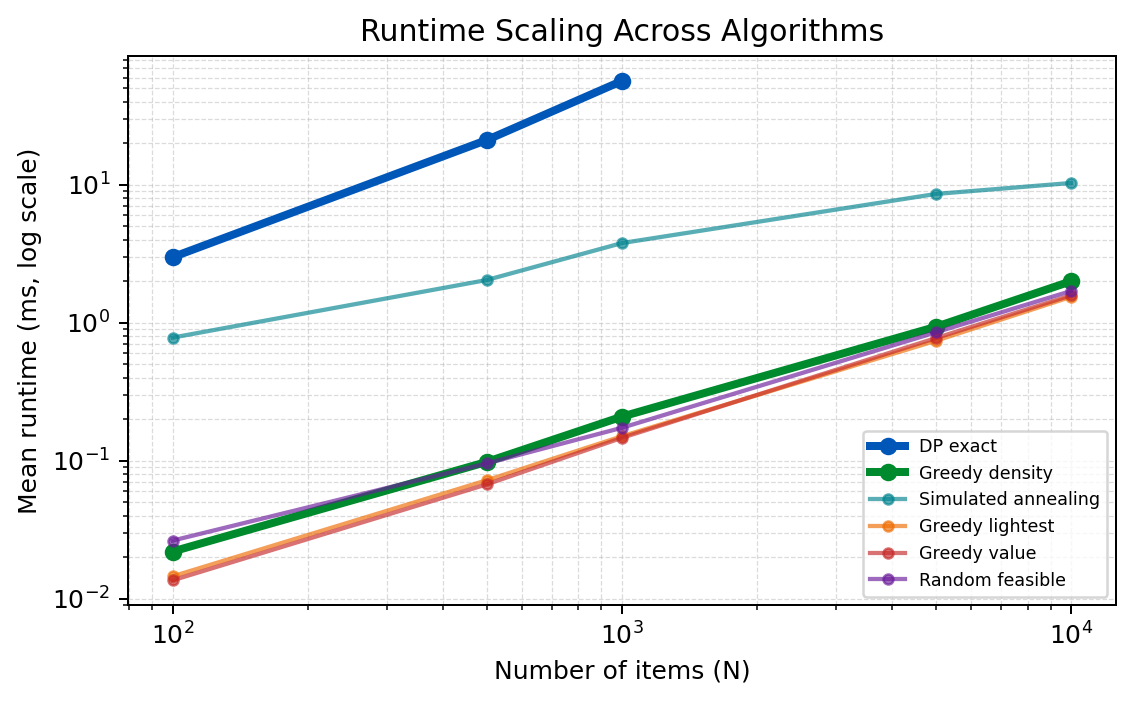
\includegraphics[width=\columnwidth]{figures/runtime_scaling.png}
\caption{Runtime scaling of exact and heuristic algorithms across problem sizes.}
\label{fig:runtime-scaling}
\end{figure}

Figure \ref{fig:gap-comparison} shows the approximation gap for $N=1000$. Greedy density is visually almost indistinguishable from DP in terms of objective value, while greedy value and random feasible selection lose a large portion of the optimum. This is the most important quality comparison: not every fast heuristic is equally reliable.

\begin{figure}[!t]
\centering
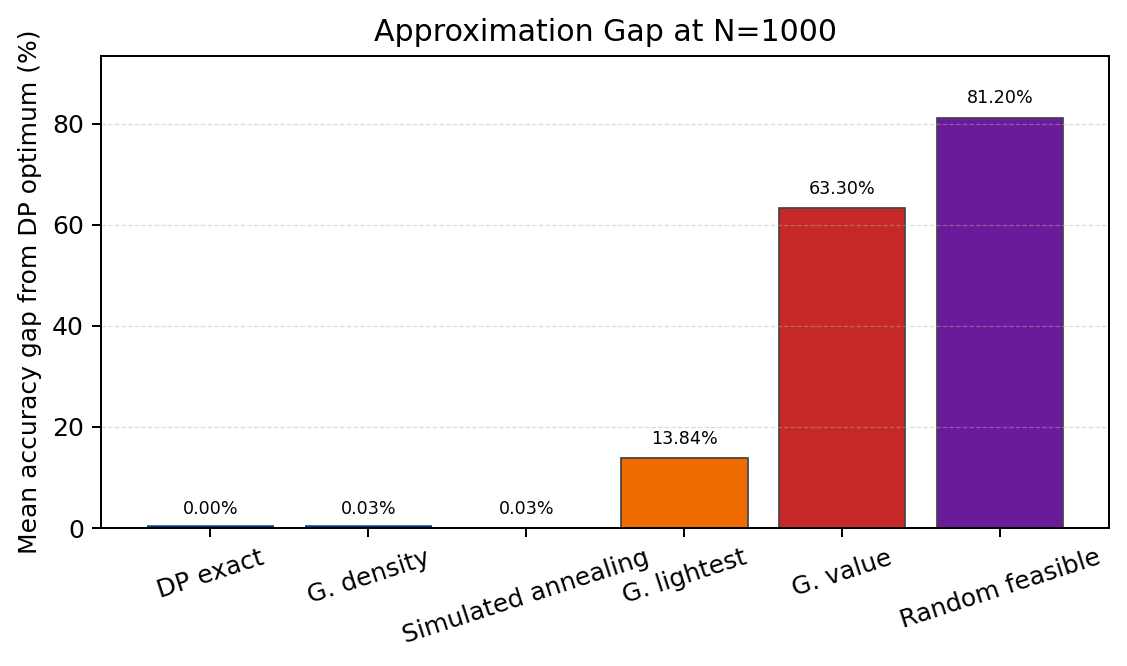
\includegraphics[width=\columnwidth]{figures/gap_comparison_n1000.png}
\caption{Mean approximation gap from the DP optimum for $N=1000$ over 100 paired runs.}
\label{fig:gap-comparison}
\end{figure}

Table \ref{tab:repeated-knapsack} reports the same repeated synthetic results numerically. For $N=100$ and $N=1000$, DP gives the optimum but is slower than greedy methods. At $N=1000$, DP takes 56.644 ms on average, while greedy density takes only 0.209 ms. However, greedy density remains very close to optimum, with only 0.03\% mean gap. Greedy value is much weaker: its mean gap reaches 63.30\% at $N=1000$.

\begin{table}[!t]
\caption{Repeated Synthetic Knapsack Results (100 Runs per Size)}
\label{tab:repeated-knapsack}
\centering
\scriptsize
\resizebox{\columnwidth}{!}{%
\begin{tabular}{@{}llrrrr@{}}
\toprule
\rowcolor{tablehead}
$N$ & Algorithm & Mean Value & Mean Time (ms) & Mean Gap (\%) & Timeout Rate \\
\midrule
\rowcolor{tokenpackhighlight}100 & \textbf{DP exact} & 35491.8 & 2.991 & 0.00 & 0.00 \\
\rowcolor{tokenpackhighlight}100 & \textbf{Greedy density} & 35439.0 & 0.022 & 0.15 & 0.00 \\
100 & Greedy value & 31962.1 & 0.014 & 9.95 & 0.00 \\
100 & Random feasible & 20124.2 & 0.026 & 43.35 & 0.00 \\
100 & Simulated annealing & 35439.8 & 0.781 & 0.15 & 0.00 \\
\rowcolor{tokenpackhighlight}1000 & \textbf{DP exact} & 111281.2 & 56.644 & 0.00 & 0.00 \\
\rowcolor{tokenpackhighlight}1000 & \textbf{Greedy density} & 111252.4 & 0.209 & 0.03 & 0.00 \\
1000 & Greedy value & 40785.1 & 0.147 & 63.30 & 0.00 \\
1000 & Random feasible & 20897.2 & 0.173 & 81.20 & 0.00 \\
1000 & Simulated annealing & 111252.4 & 3.784 & 0.03 & 0.00 \\
\rowcolor{tokenpackhighlight}10000 & \textbf{DP exact} & -- & -- & -- & 1.00 \\
\rowcolor{tokenpackhighlight}10000 & \textbf{Greedy density} & 342178.6 & 2.001 & -- & 0.00 \\
10000 & Greedy value & 43537.4 & 1.582 & -- & 0.00 \\
10000 & Random feasible & 21552.6 & 1.701 & -- & 0.00 \\
10000 & Simulated annealing & 342178.6 & 10.320 & -- & 0.00 \\
\bottomrule
\end{tabular}%
}
\end{table}


Figure \ref{fig:dp-scalability} shows why DP cannot be used blindly on very large candidate pools. The x-axis is the DP state space $nC$. The red timeout points appear after the configured state threshold. This directly illustrates the pseudo-polynomial limitation of the exact method.

\begin{figure}[!t]
\centering
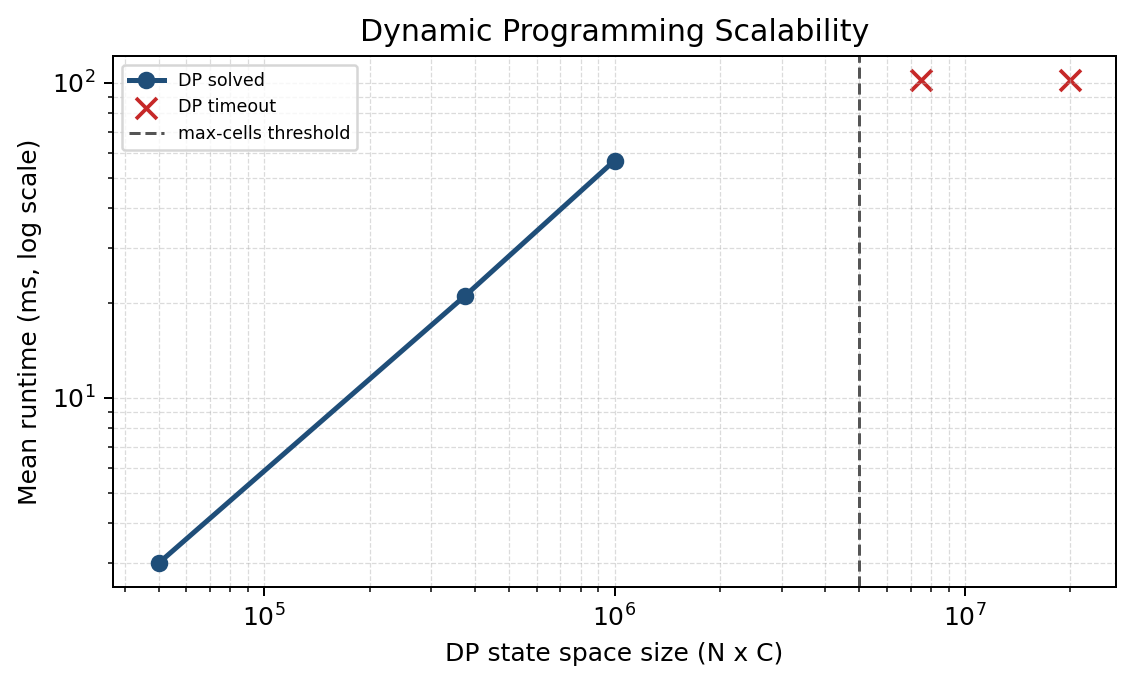
\includegraphics[width=\columnwidth]{figures/dp_state_scalability.png}
\caption{Dynamic programming runtime and timeout behavior as the $nC$ state space grows.}
\label{fig:dp-scalability}
\end{figure}

Table \ref{tab:dp-scalability} gives the exact state counts behind Figure \ref{fig:dp-scalability}. DP works for 50,000, 375,000, and 1,000,000 states in this experiment, but it is skipped at 7,500,000 and 20,000,000 states. This directly demonstrates the pseudo-polynomial limitation of dynamic programming.

\begin{table}[htbp]
\caption{DP Scalability as $nC$ Grows}
\label{tab:dp-scalability}
\centering
\begin{tabular}{@{}rrrr@{}}
\toprule
\rowcolor{tablehead}
$N$ & Capacity & $nC$ States & Timeout Rate \\
\midrule
100 & 500 & 50000 & 0.00 \\
500 & 750 & 375000 & 0.00 \\
1000 & 1000 & 1000000 & 0.00 \\
5000 & 1500 & 7500000 & 1.00 \\
10000 & 2000 & 20000000 & 1.00 \\
\bottomrule
\end{tabular}
\end{table}


\begin{table}[htbp]
\caption{Retrieval Feasibility With and Without TokenPack}
\label{tab:retrieval-feasibility}
\centering
\scriptsize
\begin{tabular}{rlrrr}
\hline
Eff. Budget & Method & Recall & Avg. Tokens & Over Budget \\
\hline
250 & document-prefix & 0.25 & 180 & 0.00 \\
250 & full-document & 1.00 & 1539 & 1.00 \\
250 & top-k & 0.94 & 809 & 1.00 \\
\rowcolor{tokenpackhighlight}250 & \textbf{TokenPack knapsack} & \textbf{0.75} & \textbf{213} & \textbf{0.00} \\
700 & document-prefix & 0.69 & 698 & 0.00 \\
700 & full-document & 1.00 & 1539 & 1.00 \\
700 & top-k & 0.94 & 809 & 0.88 \\
\rowcolor{tokenpackhighlight}700 & \textbf{TokenPack knapsack} & \textbf{0.94} & \textbf{657} & \textbf{0.00} \\
\hline
\end{tabular}
\end{table}
\FloatBarrier

Table \ref{tab:retrieval-feasibility} shows why TokenPack improves the process rather than only adding implementation complexity. Without TokenPack, the document-prefix baseline is budget-valid but misses much of the evidence. The full-document baseline reaches perfect recall only by violating the budget. Plain top-k is semantically strong but also frequently over budget. Knapsack selection gives the desired middle point: high evidence recall while keeping the selected context inside the effective token capacity.

\begin{table}[!t]
\caption{LLM Answer Quality Pilot (Review-Aware)}
\label{tab:llm-answer-quality}
\centering
\scriptsize
\resizebox{\columnwidth}{!}{%
\begin{tabular}{llrrrrl}
\hline
Model & Strategy & Completed & Invalid & Avg. Tokens & Avg. Score & Source \\
\hline
Large cloud & document-prefix & 8 & 0 & 698.0 & 0.75 & auto-lexical \\
\rowcolor{tokenpackhighlight}Large cloud & \textbf{TokenPack knapsack} & 8 & 0 & 657.0 & 1.25 & auto-lexical \\
Large cloud & top-k & 1 & 7 & 808.8 & 0.00 & auto-lexical \\
Medium local & document-prefix & 8 & 0 & 698.0 & 1.75 & auto-lexical \\
\rowcolor{tokenpackhighlight}Medium local & \textbf{TokenPack knapsack} & 8 & 0 & 657.0 & 2.00 & auto-lexical \\
Medium local & top-k & 1 & 7 & 808.8 & 2.00 & auto-lexical \\
Small local & document-prefix & 8 & 0 & 698.0 & 1.12 & auto-lexical \\
\rowcolor{tokenpackhighlight}Small local & \textbf{TokenPack knapsack} & 8 & 0 & 657.0 & 1.00 & auto-lexical \\
Small local & top-k & 1 & 7 & 808.8 & 2.00 & auto-lexical \\
\hline
\end{tabular}%
}
\end{table}


Table \ref{tab:llm-answer-quality} adds a model-output perspective. The small local model is weak and should be interpreted carefully, but the medium model shows the intended pattern: TokenPack knapsack completes all valid prompts and reaches the strongest pilot score, while top-k completes only one prompt because most top-k selections exceed the token budget.

\begin{table}[!t]
\caption{Estimated Input Cost Savings From LongBench v2 Context Reduction}
\label{tab:cost-savings}
\centering
\scriptsize
\begin{tabular}{@{}lrrr@{}}
\toprule
\rowcolor{tablehead}
Method & Paid Tokens & Cost (\$) & Saving vs Full Doc \\
\midrule
Full context & 1000000 & 2.500 & 0.0\% \\
\rowcolor{tokenpackhighlight}\textbf{TP-50} & \textbf{495725} & \textbf{1.239} & \textbf{50.4\%} \\
LLL-0.50 & 487808 & 1.220 & 51.2\% \\
\rowcolor{tokenpackhighlight}\textbf{TP-50 + LLL-0.50} & \textbf{255218} & \textbf{0.638} & \textbf{74.5\%} \\
\bottomrule
\end{tabular}
\end{table}


\begin{figure}[!t]
\centering
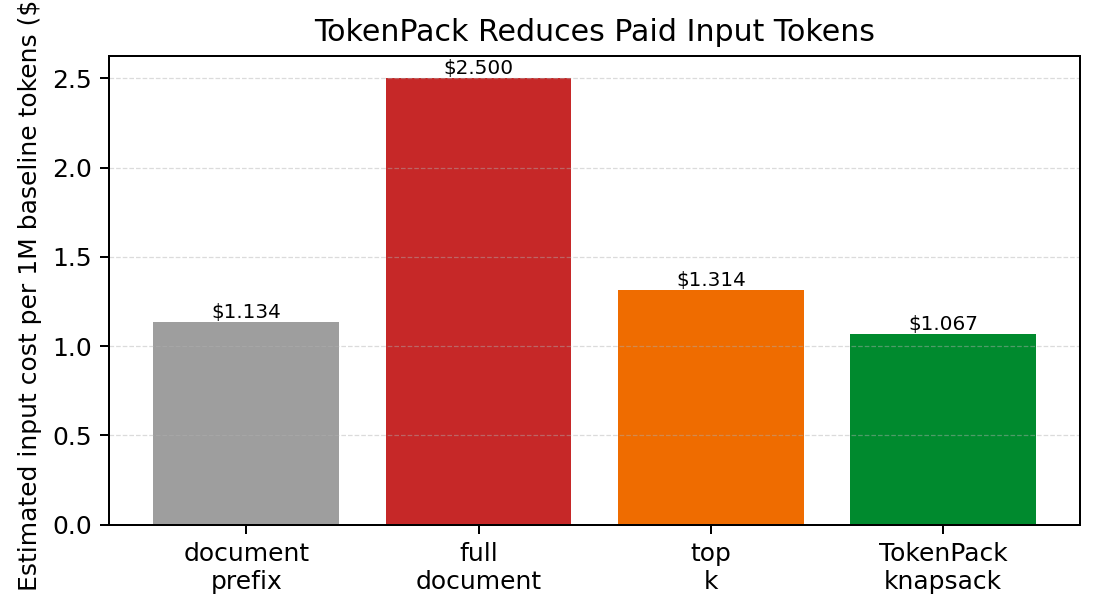
\includegraphics[width=\columnwidth]{figures/tokenpack_cost_savings.png}
\caption{Estimated input-token cost under a 1M baseline-token scenario.}
\label{fig:cost-savings}
\end{figure}

Table \ref{tab:cost-savings} and Figure \ref{fig:cost-savings} show the economic implication of budget-aware context packing. In this scenario, TokenPack knapsack reduces paid input tokens from 1,000,000 to 426,901, corresponding to an estimated 57.3\% input-cost reduction versus full-document prompting. The exact dollar value changes with provider pricing, but the token reduction ratio is determined by the selection strategy.

\section{Discussion}
The experiments support four observations. First, exact DP is the most reliable method when the instance size is manageable because it gives the optimum. Second, the $O(nC)$ cost becomes a real limitation as the state space grows. Third, greedy density is a strong practical heuristic because it is fast and close to optimum on the tested random instances. Fourth, value-only greedy can fail badly, even though it sounds intuitive, because it ignores weight.

For LLM context selection, these observations imply that TokenPack should not run DP over every chunk in a huge corpus. Instead, the retrieval system should first create a candidate pool using embeddings, then apply DP or density-greedy selection inside that smaller pool. This hybrid design aligns with both algorithm analysis and real LLM engineering constraints. The LLM pilot reinforces the same point: TokenPack does not make the language model itself smarter; it makes the input selection process safer and more cost-efficient.

\section{Limitations and Future Work}
The current results are strongest on synthetic knapsack instances and feasibility-oriented retrieval tests. A larger manually reviewed gold-evidence dataset would be needed to prove end-to-end question answering quality. The LLM answer-quality table is a pilot and should be treated as weaker than the algorithmic benchmark unless all answer rows are manually reviewed. Future work can add genetic algorithms, branch-and-bound, and FPTAS baselines. Another useful extension is to run the retrieval benchmark on manually labeled PDF questions and compare evidence recall across multiple token budgets.

\section{Conclusion}
This project models LLM context selection as a 0/1 Knapsack Problem and evaluates exact and heuristic algorithms. The results show that simple retrieval approaches such as top-k do not guarantee token-budget feasibility, while knapsack-based selection strictly preserves the budget constraint. Repeated synthetic experiments confirm that DP gives optimal results for manageable instances but becomes costly as $nC$ grows. Greedy density is fast and often close to optimal, while value-only greedy may produce large accuracy gaps. Overall, the methodology is suitable because LLM context selection has the same structure as knapsack: maximize total utility under a strict capacity constraint.

\section*{Acknowledgment}
This work was prepared for the Algorithm Analysis and Design course.

\bibliographystyle{IEEEtran}
\bibliography{references}

\end{document}
